\chapter{Joint profiling of chromatin accessibility DNA methylation and transcription in single cells}
\graphicspath{{Chapter1/Figs/}}

(COPIED FROM ABSTRACT, IS THIS OK?) Single-cell profiling techniques have provided an unprecented opportunity to study cellular heterogeneity at multiple molecular levels. The maturation of single-cell RNA-sequencing technologies has enabled the identification of transcriptional profiles associated with lineage diversification and cell fate commitment. Yet, the accompanying epigenetic changes and the role of other molecular layers in driving cell fate decisions remains poorly understood. Consequently, the profiling the epigenome at the single-cell level is receiving increasing attention, but without associated transcriptomic readouts, the conclusions that can be extracted from epigenetic measurements are limited.\\
%Technological advances enabled multiple biological layers to be probed in parallel at the single-cell level, unveling a powerful approach for investigating regulatory relationships. Such single-cell multi-modal technologies can reveal multiple dimensions of cellular heterogeneity and uncover how this variation is coupled between the different molecular layers, hence enabling a more profound mechanistic insight than can be inferred by analysing a single data modality in separate cells. \\

In this chapter we will describe scNMT-seq, an experimental protocol for genome-wide profiling of RNA expression, DNA methylation and chromatin accessibility in single cells. First, we will assess the quality of the triple omics readouts, followed by a comparison with similar available technologies. Subsequently, we will showcase how scNMT-seq can be used to study coordinated epigenetic and transcriptomic heterogeneity along a differentiation process. \\

The work discussed in this chapter results from a collaboration with the Wolf Reik lab (Babraham Institute, Cambridge, UK). It has been peer-reviewed and published in Clark \& Argelaguet et al \cite{Clark2018}.\\
The methodology was conceived by Stephen Clark, who performed most of the experiments. Felix Krueger processed and managed sequencing data. I performed the computational analysis, except for the reconsutraction of chromatin accessibility profiles, which was done by Andreas Kapourani. Guido Sanguinetti, Gavin Kelsey, John C. Marioni, Oliver Stegle and Wolf Reik supervised the project.\\
The article was jointly written by Stephen Clark, John Marioni, Oliver Stegle and Wolf Reik, and me.

\section{Description of the experimental protocol}
scNMT-seq builds on two previous multi-modal single-cell sequencing protocols: single-cell Methylation and Transcriptome sequencing (scM\&T-seq) \cite{Angermueller2016} and Nucleosome Occupancy and Methylation sequencing (NOMe-seq) \cite{Kelly2012,Pott2016}.\\
In a first step (the NOME-seq step), cells are sorted into individual wells and incubated with a GpC methyltransferase (M.CviPI). As shown \textit{in vitro}, this enzyme labels accessible (or nucleosome depleted) GpC sites via DNA methylation\cite{Kilgore2007, Kelly2012}. In mammalian genomes, cytosine residues in GpC dinucleotides are methylated at a very low rate. Hence, after M.CviPI treatment, GpC methylation marks can be interpreted as direct read outs for chromatin accessibility, as opposed to the CpG methylation readouts, which can be interpreted as endogenous DNA methylation\cite{Kilgore2007, Kelly2012}.\\
In a second step (the scM\&T-seq step), the DNA molecules are separated from the mRNA using oligo-dT probes pre-annealed to magnetic beads. Subsequently, the DNA fraction undergoes single-cell bisulfite conversion\cite{Smallwood2014}, whereas the RNA fraction undergoes Smart-seq2 \cite{Picelli2014}.\\

\begin{figure}[H]
	\centering
	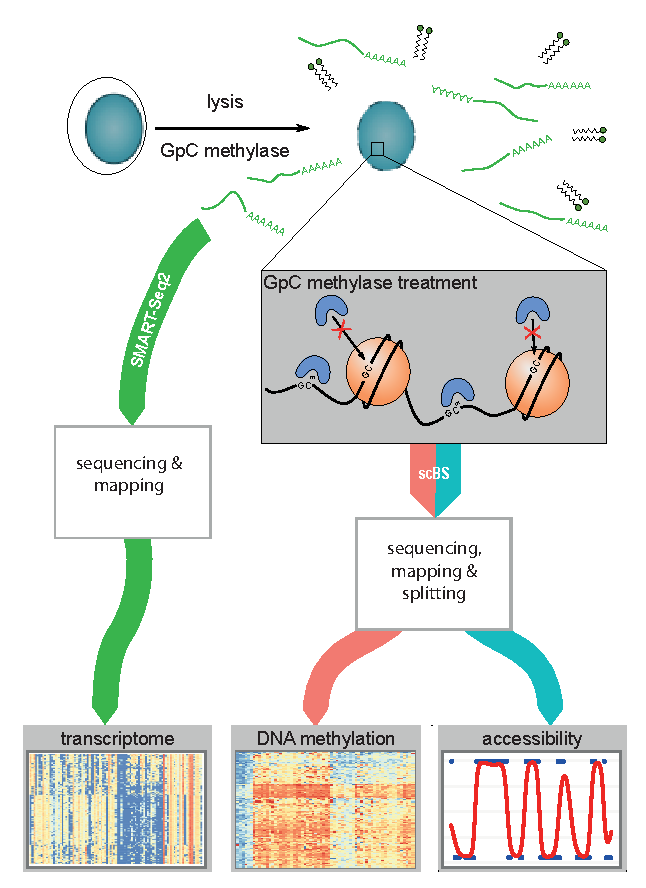
\includegraphics[width=0.6\linewidth]{scNMT_protocol}
	\caption[]{}
	\label{fig:scnmt_protocol}
\end{figure}

As discussed in [[SECTION XXX]], NOME-seq has a range of appealing properties in comparison with count-based methods such as ATAC-seq or DNAseq-seq. First, the obvious gain of simultaneously measuring another epigenetic readout such as DNA methylation with little additional cost. Second, the resolution of the method is determined by the frequency of GpC sites within the genome (\~1 in 16 bp), rather than the size of a library fragment (usually >100 bp). This allows the robust inspection of individual regulatory elements, nucleosome positioning and transcription factor footprints \cite{Kelly2012,Pott2016,Nordstrom2019}. Third, missing data can be easily discriminated from inaccessible chromatin. Importantly, this implies that lowly accessible sites will not suffer from increased technical variation (due to low read counts) compared to highly accessible sites. Finally, the M.CviPI enzyme shows less sequence motif biases than the DNAse or the Tn5 transposase \cite{Nordstrom2019}\\ 

The downsides of the approach are the limited scalability associated with plate-based methods, and the need to discard read outs from (1) GCG positions (21\%), as it is intrinsically not possible to distinguish endogenous methylation from \textit{in vitro} methylated bases, and (2) CGC positions (27\%), to mitigate off-target effects of the enzyme \cite{Kelly2012}. This filtering step reduces the number of genome-wide cytosines that can be assayed from 22 million to 11 million. 


\section{Description of the data processing pipeline}
After DNA sequencing, reads undergo quality control and trimming using TrimGalore to remove the first 6bp (the random primers), adaptor contamination and poor-quality base calls. Subsequently, trimmed reads are aligned to the corresponding genome assembly. Here we used Bismark \cite{Krueger2011} with the additional --NOMe option, which produces CpG report files containing only ACG and TCG trinucleotides and GpC report files containing only GCA, GCC and GCT positions.\\
After mapping, a new round of quality control is performed based on mapping efficiency, bisulfite conversion efficiency and library size.\\
Finally, methylation calls for each CpG and GpC site are extracted after removal of duplicate alignments. Following the approach of \cite{Smallwood2014}, individual CpG or GpC sites in each cell are modelled using a binomial model where the number of successes is the number of methylated reads and the number of trials is the total number of reads. A CpG methylation or GpC accessibility rate for each site and cell is calculated by maximum likelihood.\\

When quantifying DNA methylation and chromatin accessibility rates over genomic features (i.e. promoters or enhancers), a binomial node is assumed again per cell and feature, but aggregating the counts over all CpG (methylation) and GpC (accessibility) dinucleotides overlapping the genomic feature.

\section{Validation}

\subsection{Coverage}
We validated scNMT-seq using 70 EL16 mouse embryonic stem cells (ESCs) cultured in serum conditions, together with two controls: negative empty wells and three cells processed without M.CviPI enzyme treatment (i.e. using scM\&T-seq). The use of this relatively simple and well-studied \textit{in vitro} system allows us to compare DNA methylation and chromatin accessibility statistics from published data \cite{Smallwood2014,Angermueller2016,Ficz2013}.\\

First, we compared the theoretical maximum coverage with the empirical coverage. Despite the reduction in theoretical coverage due to the removal of CCG and GCG sites, we observed, for DNA methylation, a median of \~50\% of promoters, \~75\% of gene bodies and \~25\% of active enhancers captured by at least 5 CpGs in each cell. Nevertheless, limited coverage is observed for small genomic contexts such as p300 ChIP-seq peaks (median of 200bp).\\
For chromatin accessibility, coverage was larger than that observed for endogenous methylation due to the higher frequency of GpC dinucleotides, with a median of ~85\% of gene bodies and ~75\% of promoters measured with at least 5 GpCs.

\begin{figure}[H]
	\centering
	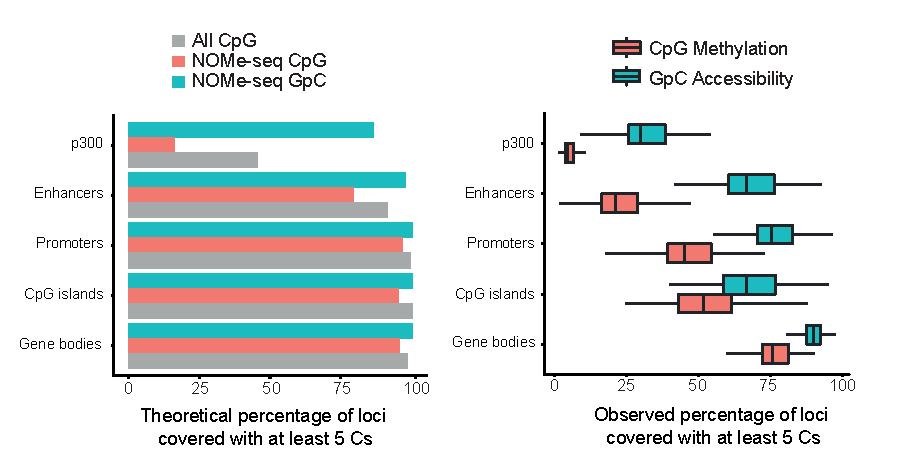
\includegraphics[width=1.0\linewidth]{scNMT_coverage}
	\caption[]{}
	\label{fig:scnmt_coverage}
\end{figure}

Next, we compared the DNA methylation coverage with previous single-cell bisulfite sequencing protocols\cite{Angermueller2016}. Despite scNMT-seq yielding less CpG measurements, we find little differences in coverage when quantifying DNA methylation over genomic contexts, albeit these become evident when down-sampling the number of reads:

\begin{figure}[H]
	\centering
	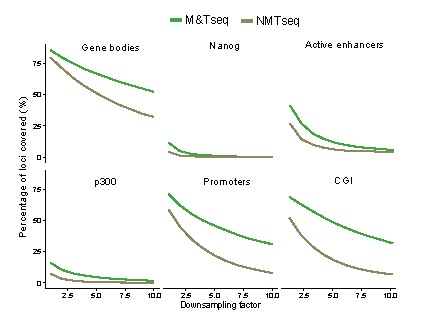
\includegraphics[width=0.8\linewidth]{scNMT_coverage2}
	\caption[]{}
	\label{fig:scnmt_coverage2}
\end{figure}




\subsection{Consistency with previous studies}

To assess consistency with previous studies we performed several comparisons.\\

First, we computationally pseudobulked the data across all cells and we examined DNA methylation and chromatin accessibility levels at loci with known regulatory roles. We found that in promoters, DNaseI hypersensitivity sites, enhancer regions and transcription factors binding sites, DNA methylation was decreased while chromatin accessibility was increased, as previously reported \cite{Pott2016}. As a control, we observe that cells which did not receive M.CviPI treatment showed globally low GpC methylation levels (~2\%).

\begin{figure}[H]
	\centering
	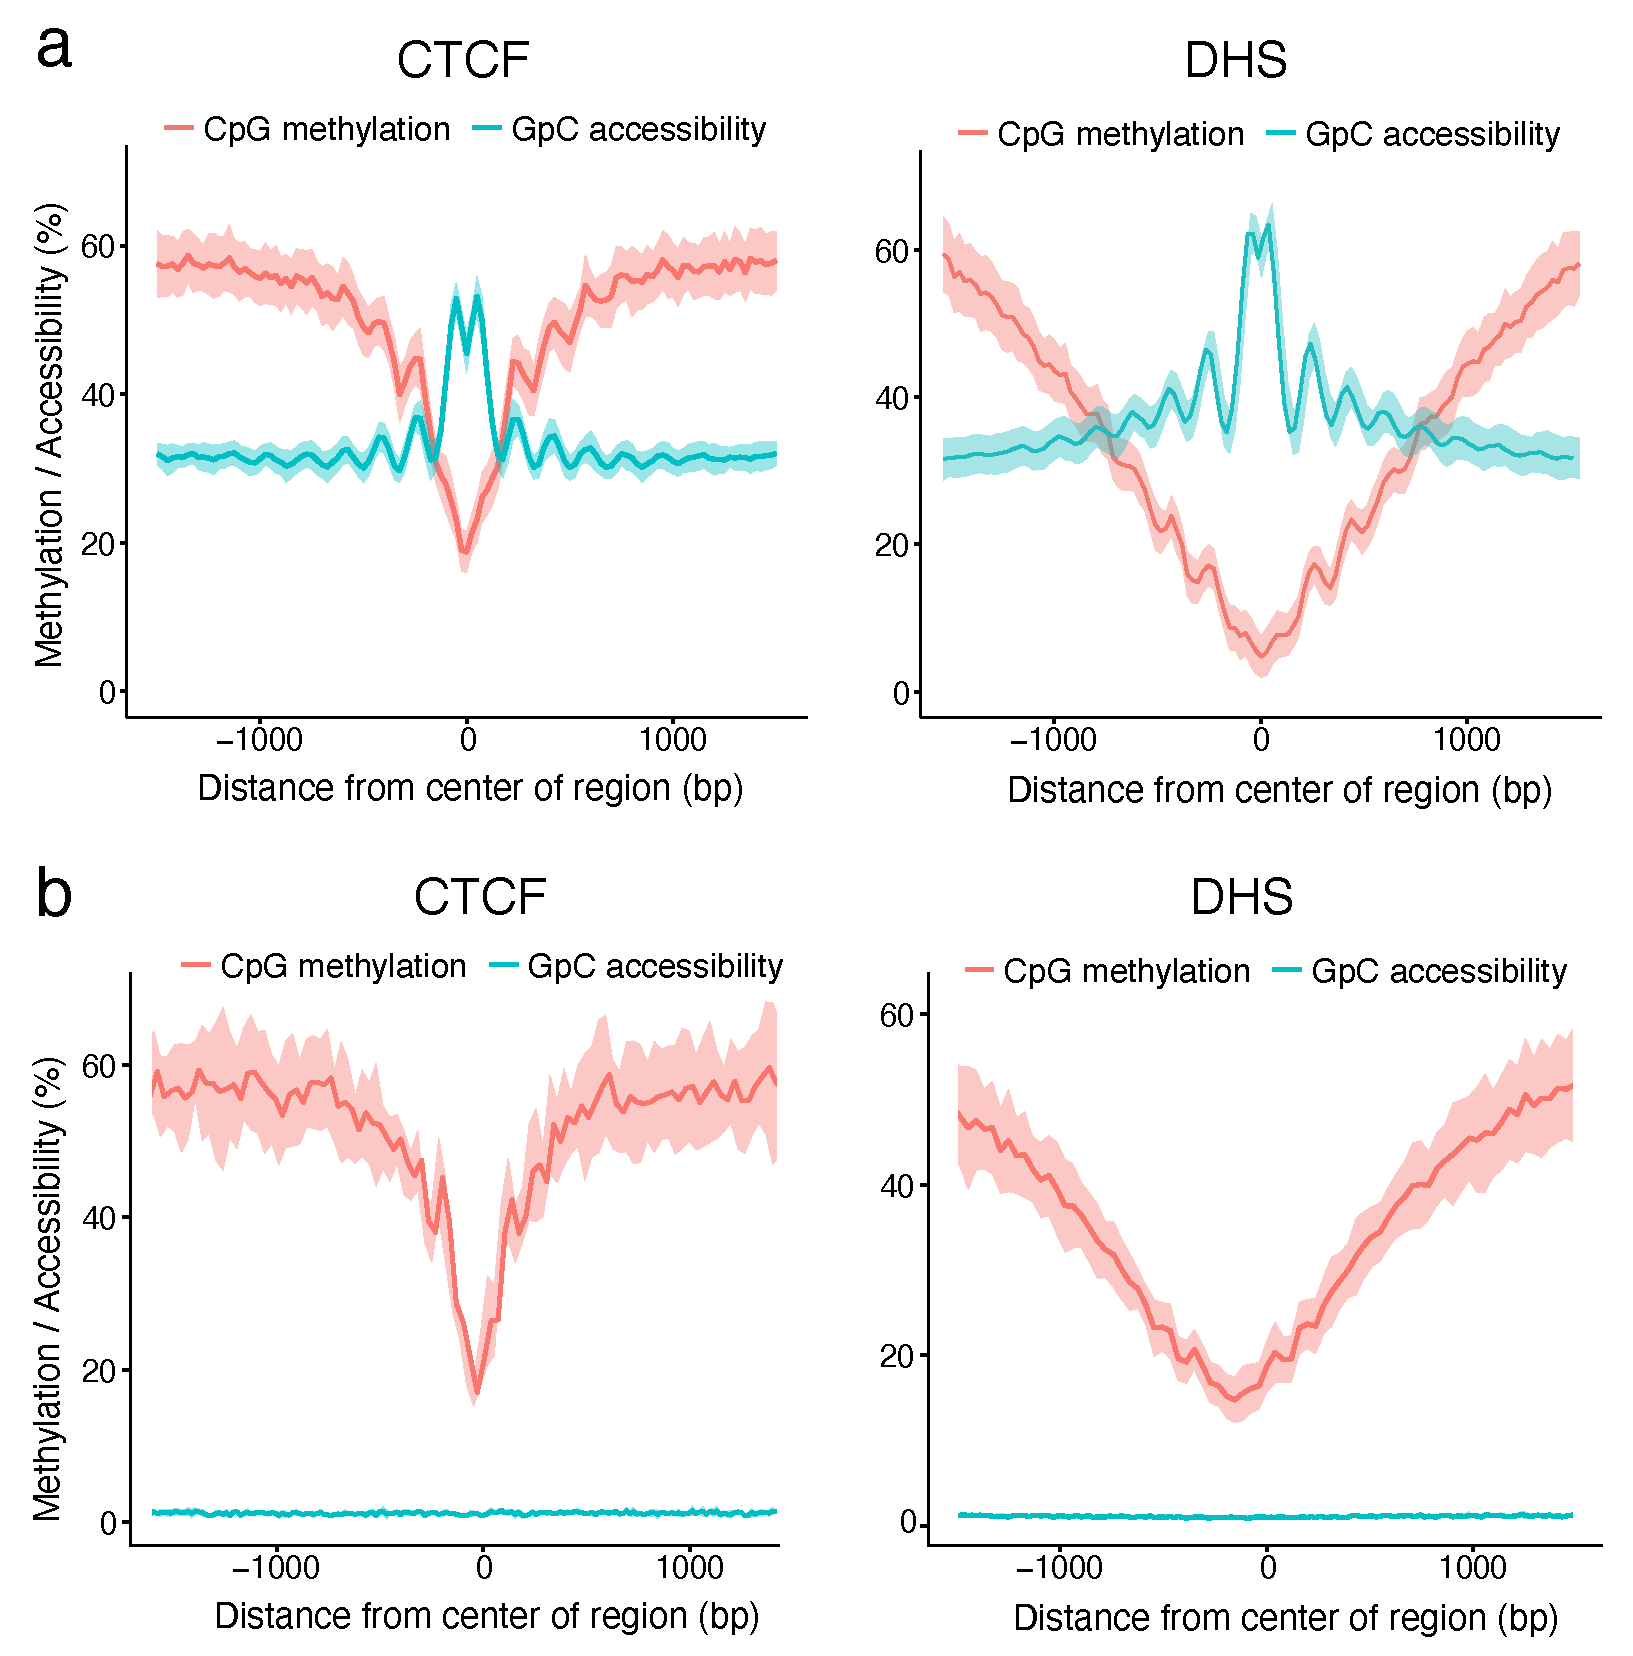
\includegraphics[width=0.8\linewidth]{scNMT_pseudobulk_profiles}
	\caption[]{}
	\label{fig:scnmt_profiles}
\end{figure}



% \begin{figure}[H]
% 	\centering
% 	\includegraphics[width=0.8\linewidth]{scNMT_profiles}
% 	\caption[]{}
% 	\label{fig:scnmt_profiles}
% \end{figure}


Second, rather than interrogating supervised annotations, we quantified DNA methylation and chromatin accessibility using a running window throughout the genome. The resulting measurements were compared to data sets from the same cell lines profiled with similar technologies, including scM\&T-seq\cite{XX}, scBS-seq\cite{XX} and bulk BS-seq\cite{XX}. When comparing the methylomes, we find that most of the variation is not attributed to the technology but to differences in culture condition.\\
Regarding accessibility, no NOME-seq measurements were available for ESCs at the time of the study, so we compared it to published bulk DNase-seq data from the same cell type, yielding good consistency between datasets (Pearson R = 0.74).
\begin{figure}[H]
	\centering
	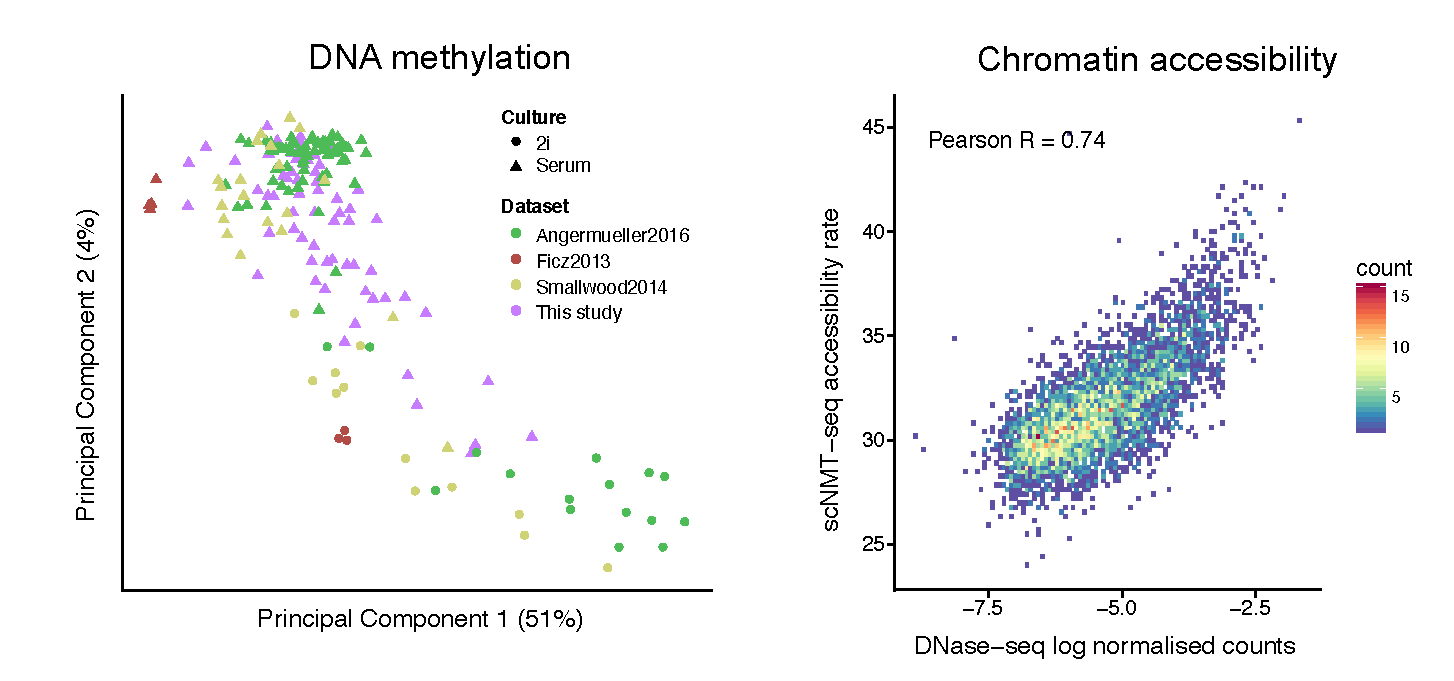
\includegraphics[width=1.0\linewidth]{scNMT_comparison}
	\caption[]{}
	\label{fig:scnmt_comparison}
\end{figure}

Finally, we attempted to reconstruct the expected relationships between the transcriptome and the epigenome, mainly the positive association between RNA expression and chromatin accessibility and the negative association between DNA methylation and RNA expression \cite{Thurman2012,Angermueller2016,XXX}. To get a measure of the coupling between two molecular layers, we simply performed a linear association (Pearson correlation) per cell (across genes). Notice that this approach is not exclusive to single-cell data and can be computed (more accurately) with bulk measurements. Reassuringly, this analysis confirmed, within single cells, the expected positive correlation between chromatin accessibility and RNA expression, and the negative correlations between RNA expression and DNA methylation, as well as between DNA methylation and chromatin accessibility.

\begin{figure}[H]
	\centering
	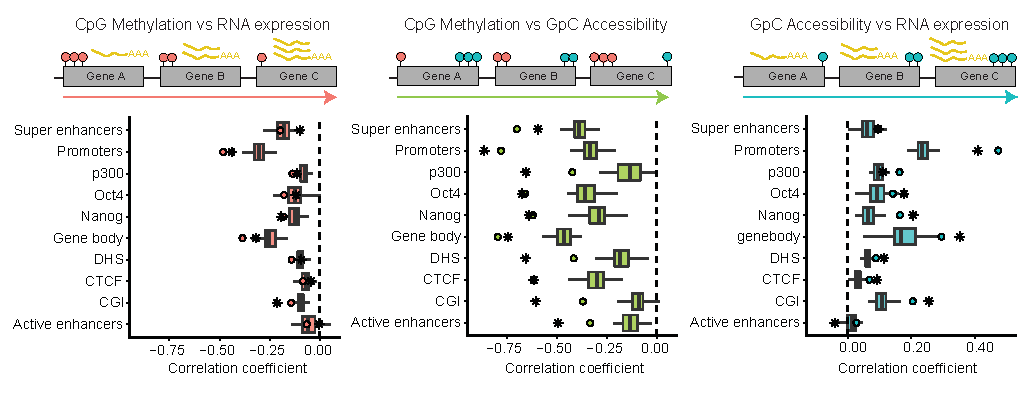
\includegraphics[width=1.0\linewidth]{scNMT_correlations_acrossgenes}
	\caption[]{}
	\label{fig:scNMT_correlations_acrossgenes}
\end{figure}


Consistently, when stratifiying the loci from Figure X based on the expression level of the nearest gene, we observe that higher RNA expression is associated with chromatin openess and decreased DNA methylation levels. 
\begin{figure}[H]
	\centering
	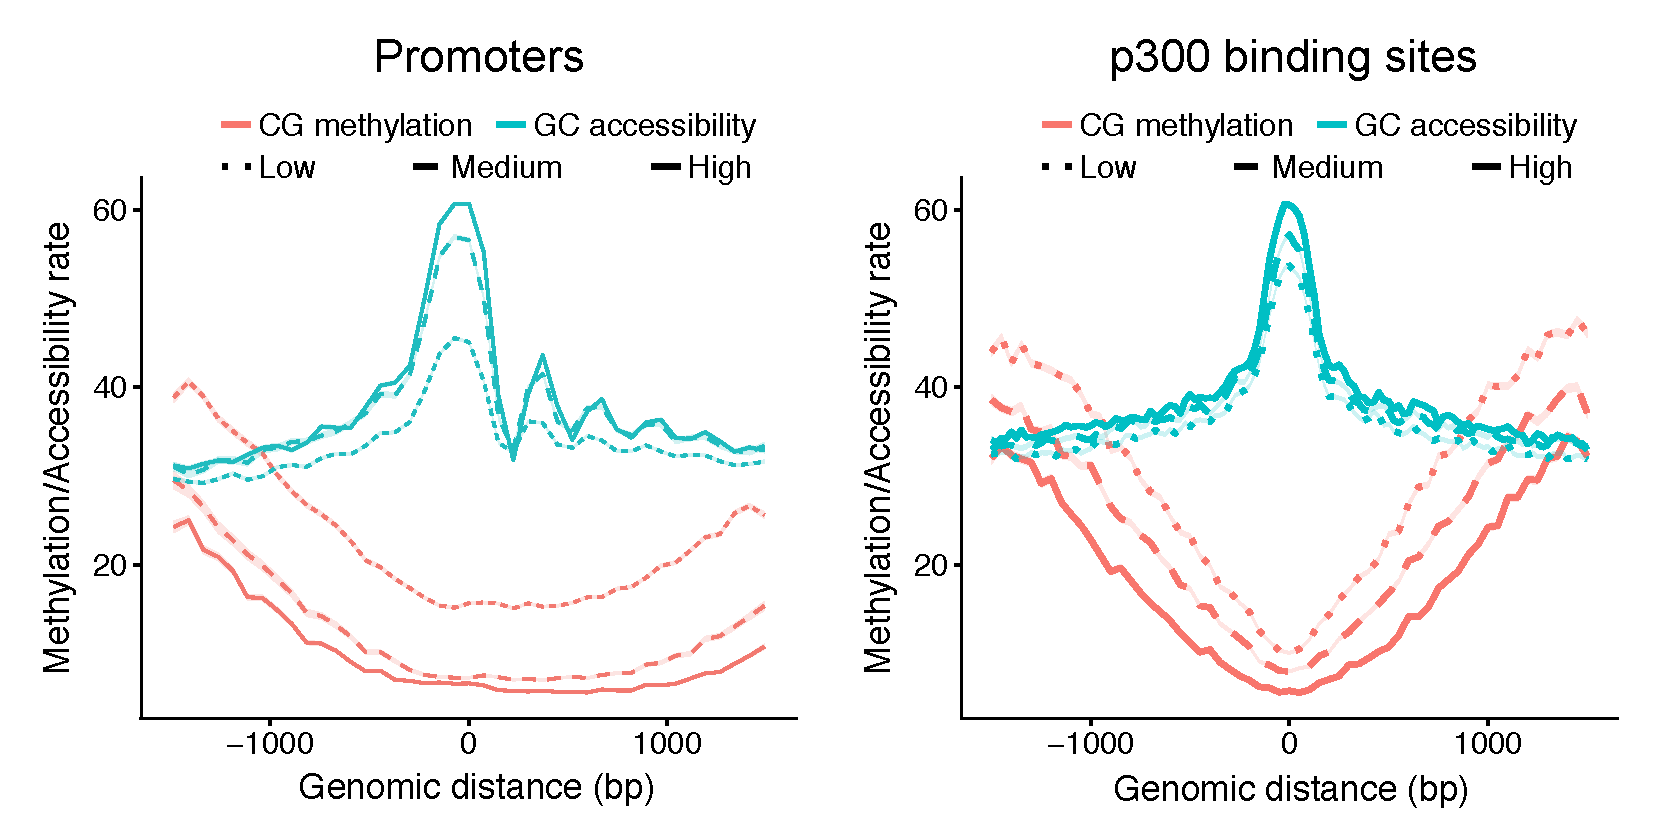
\includegraphics[width=1.0\linewidth]{scNMT_pseudobulk_profiles_byexpr}
	\caption[]{}
	\label{fig:scnmt_pseudobulk_profiles_byexpr}
\end{figure}


\section{Identification of genomic elements with coordinated variability across molecular layers}

Having validated the quality of scNMT-seq data, we next explored its potential to identify coordinated heterogeneity across different molecular layers.\\
We generated a second data set of 43 embryonic stem cells (after QC), where we induced a differentiation process towards embryoid bodies by removing the LIF media for 3 days:

\begin{figure}[H]
	\centering
	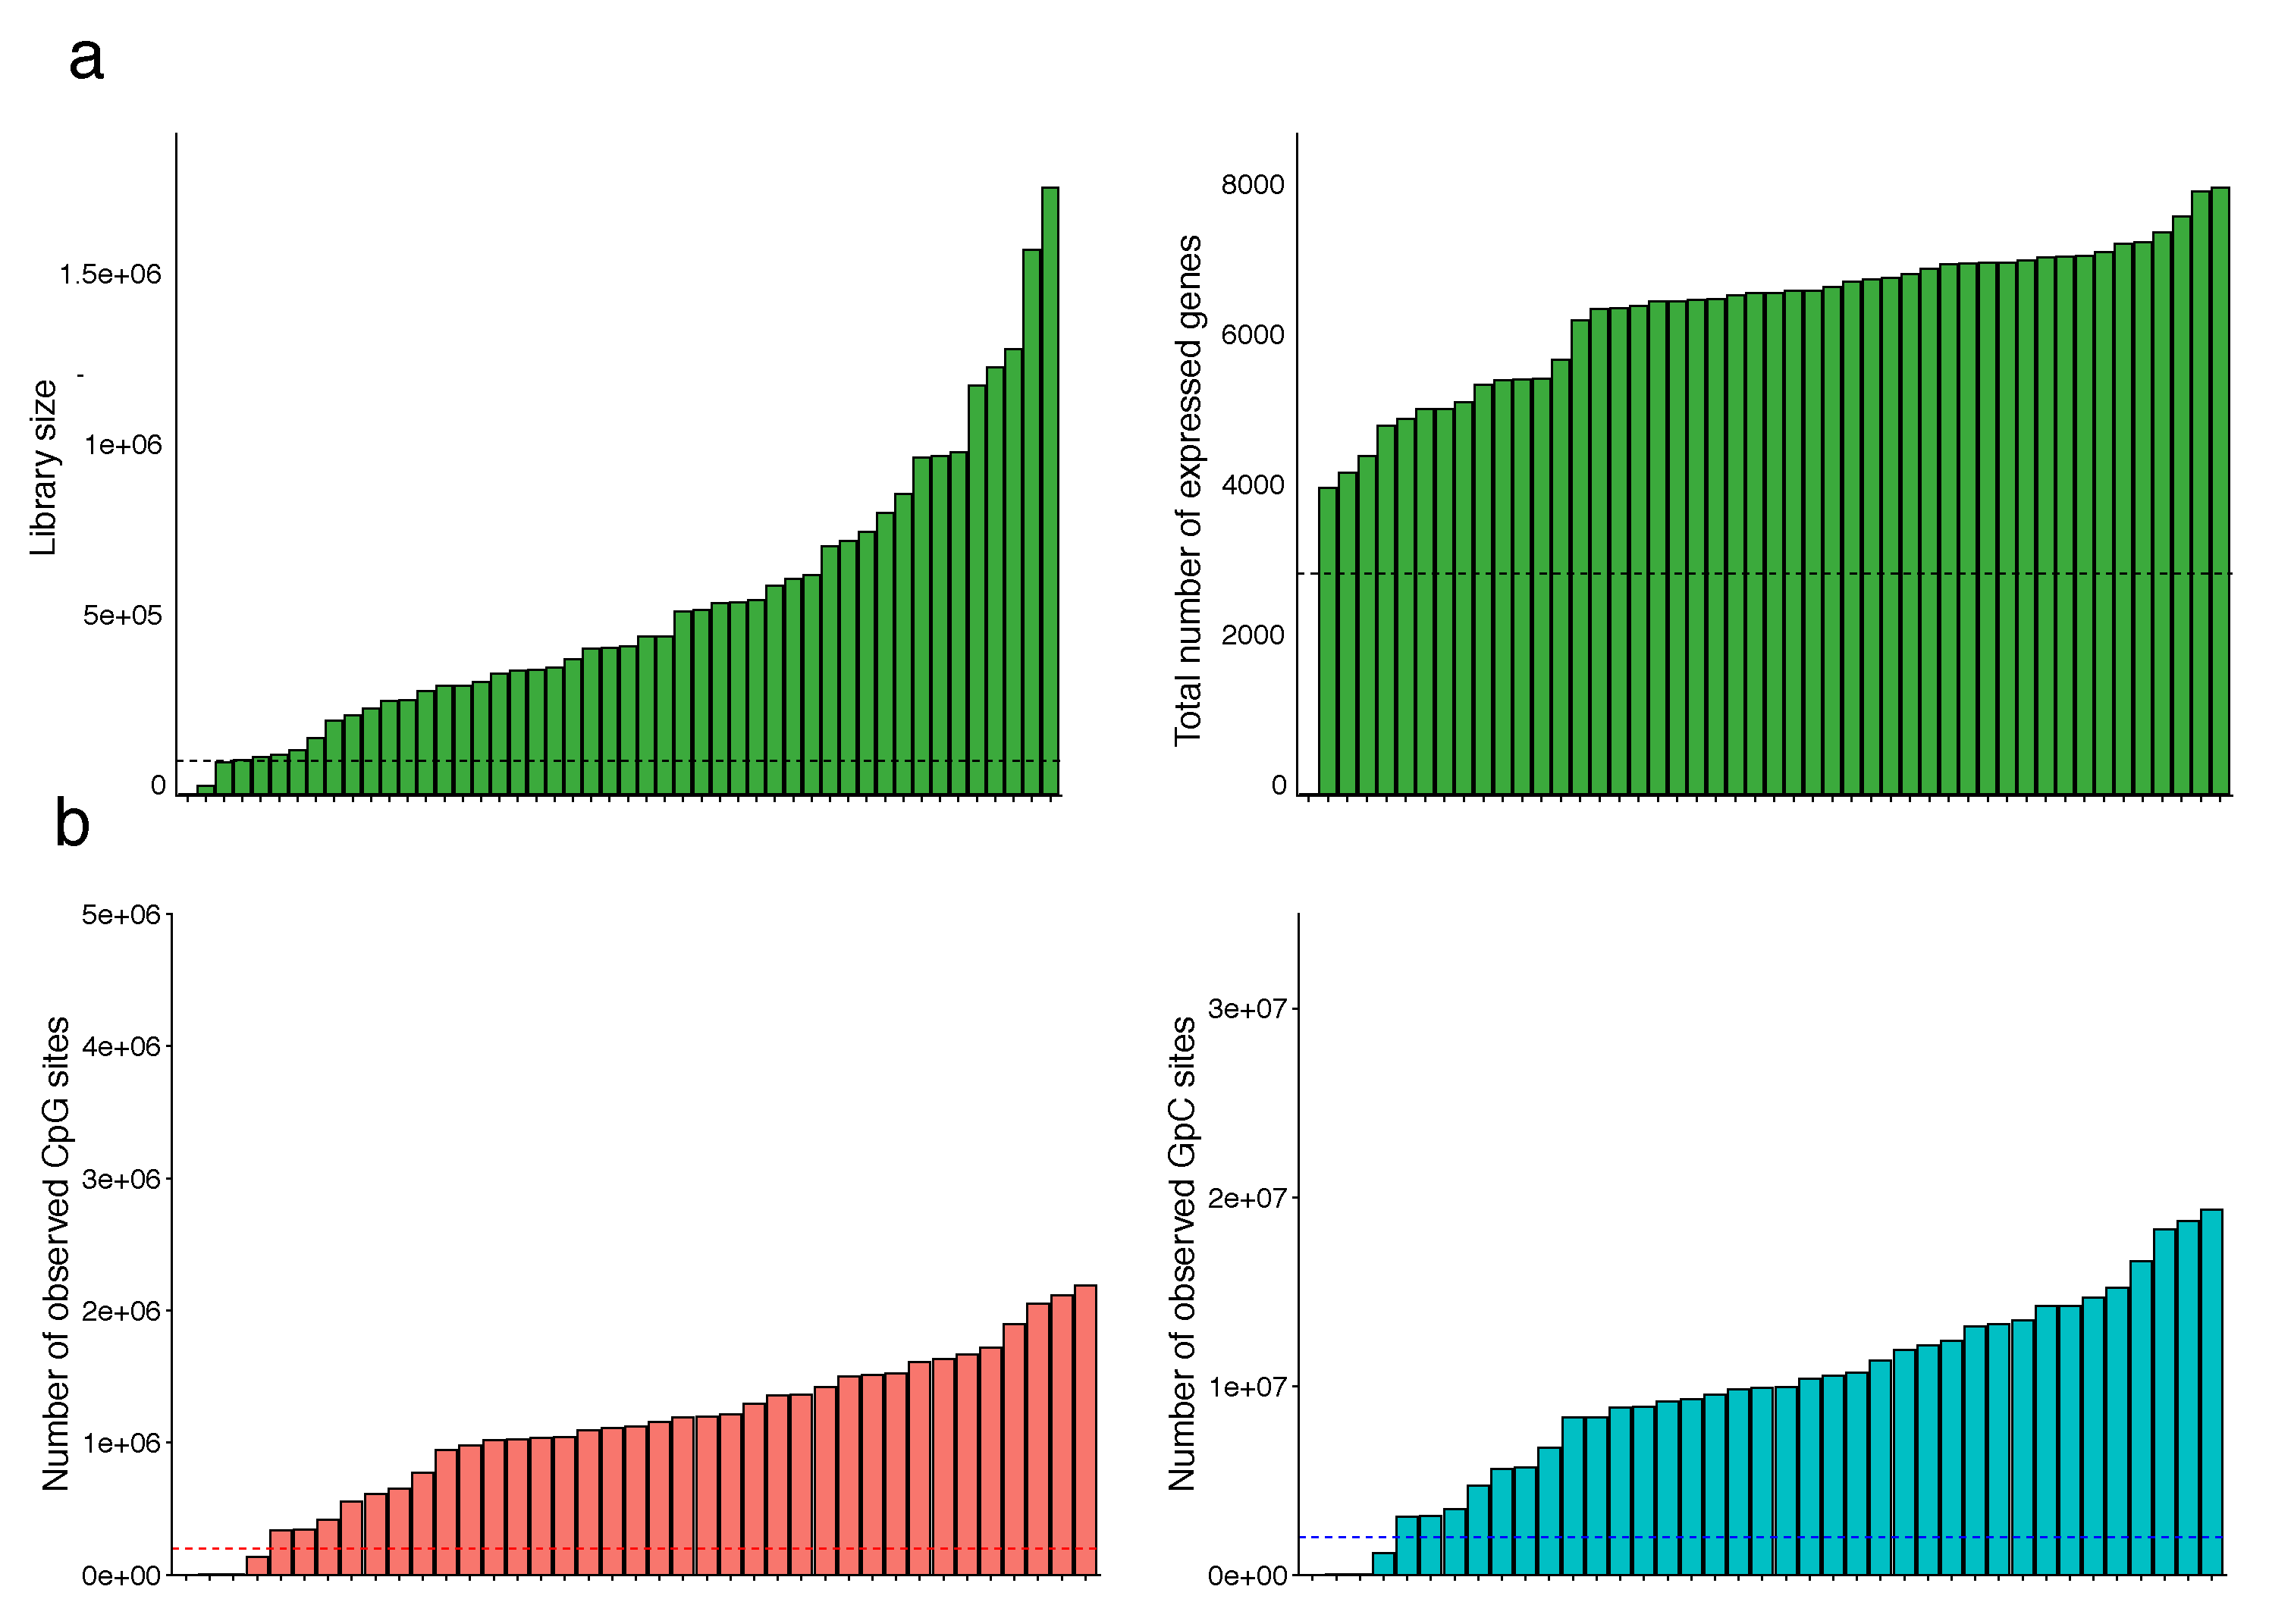
\includegraphics[width=0.8\linewidth]{scNMT_EB_QC}
	\caption[]{}
	\label{fig:scnmt_eb_qc}
\end{figure}

Dimensionality reduction on the RNA expression data reveals the existence of two subpopulations: one with high expression of pluripotency markers (Esrrb and Rex1) and the other with high expression of differentiation markers (T and Prtg). This confirms the existence of significant phenotypic heterogeneity that is required for an association analysis.

\begin{figure}[H]
	\centering
	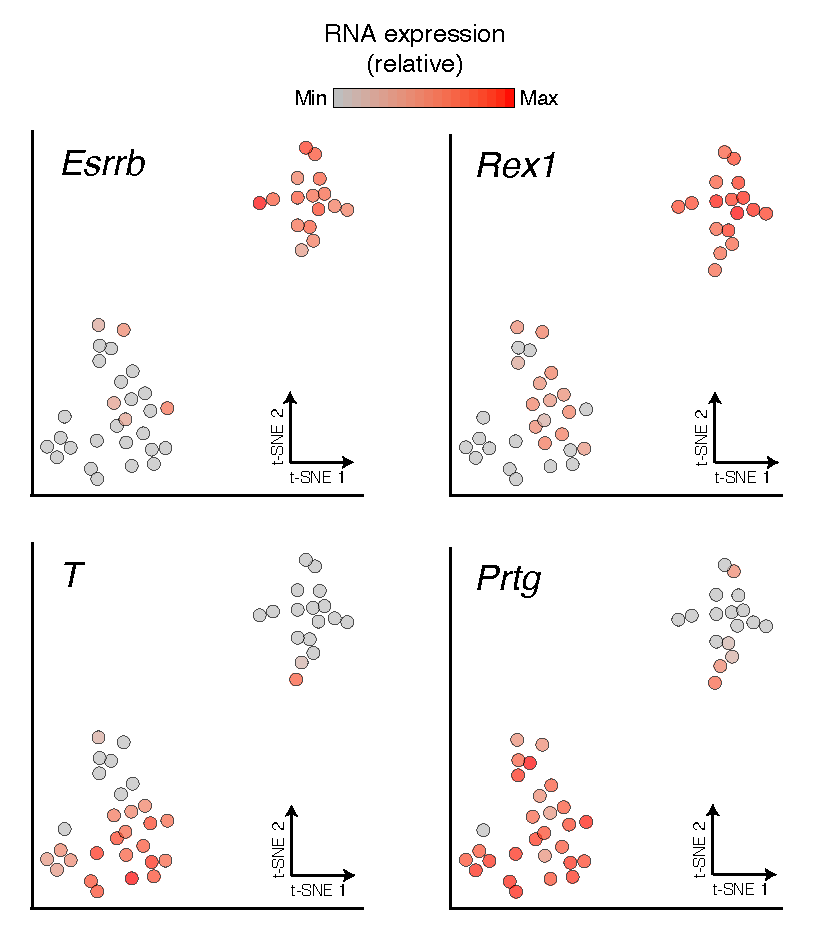
\includegraphics[width=0.8\linewidth]{scNMT_EB_RNA}
	\caption[]{}
	\label{fig:scnmt_eb_rna}
\end{figure}

Next, we tested locus-specific linear associations (across cells) between pairwise combinations of molecular layers, using the average CpG rate and GpC rate within a loci as a metric for DNA methylation and chromatin accessibility, respectively.\\
First, considering correlations between DNA methylation and RNA expression, we identified a majority of negative associations, reflecting the known relationship between these two layers. In contrast, we obtained largely positive associations between chromatin accessibility and RNA expression, mainly in promoters, p300 binding sites and super enhancer regions. Finally, we found mostly negative associations between DNA methylation and chromatin accessibility, as previously reported \cite{XX}.\\
Again, this confirms the expected direction of association between molecular layers, as reported in bulk studies. Yet, the single-cell measurements allow us to inspect the dynamics of single loci (across cells). As an illustrative example, we display the Estrogen Related Receptor Beta (Esrrb) locus, a gene involved in early development and pluripotency \cite{Papp2012}. A previous study \cite{Angermueller2016}, identified a super enhancer near Esrrb that showed high degree of correlation between DNA methylation and associated RNA expression changes. In our study, we find Esrrb to be expressed primarily in the pluripotent cells, consistent with its role in early development. When examining the epigenetic dynamics of the corresponding super enhancers, we observe a strong negative correlation between DNA methylation and RNA expression, hence replicating previous findings. Additionally, we observe a strong negative relationship between DNA methylation and chromatin accesibility, indicating the two epigenetic layers are tightly coupled, consistent with the correlations per cell (across genes), displayed in Figure X.

\begin{figure}[H]
	\centering
	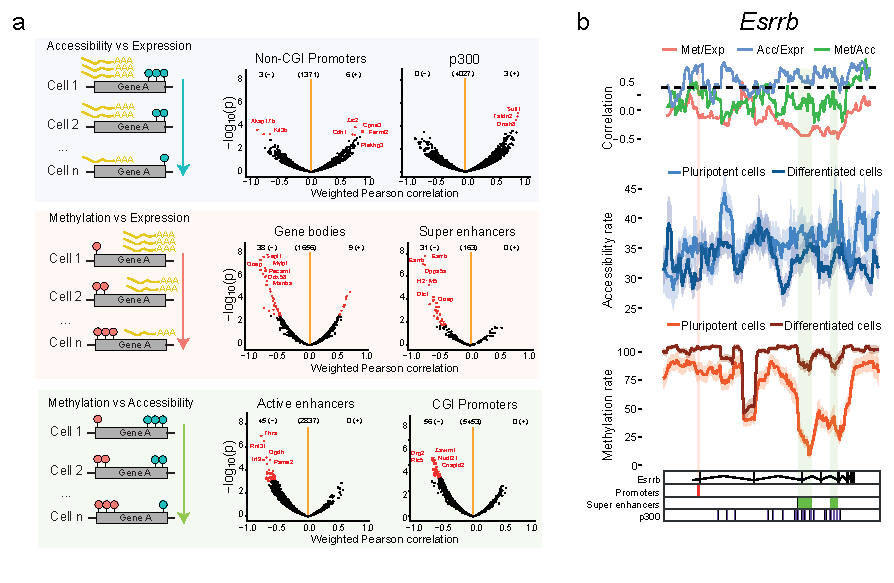
\includegraphics[width=0.9\linewidth]{scNMT_EB_correlations}
	\caption[]{}
	\label{fig:scnmt_eb_correlations}
\end{figure}


\section{Inference of non-linear chromatin accessibility profiles at the base pair resolution}
A clear advantage of scNMT-seq, compared to other chromatin accessibility technologies, is the high resolution of the its readouts, namely a binary output for each observed GpC dinucleotide. As illustrated in Figure 1, GpC accessibility measurements show complex oscillatory patterns, likely due to presence of nucleosomes, which are not appropriately captured by using an average rate. Therefore, we next attempted to exploit this high-resolution information to infer non-linear chromatin accessibility profiles at individual promoters.\\
(EXPLAIN BETTER) The approach we followed is based on BPRMeth \cite{Kapourani2018}, a generalized linear regression model with gaussian basis functions, coupled with a Bernoulli likelihood. A model was fit for every gene and every cell, provided enough coverage (at least 10 GpC sites observed per gene across 40\% of cells).\\
 Examples of infered regression patterns are shown in Figure X, showing significant heterogeneity in both the position and the number of nucleosomes:

\begin{figure}[H]
	\centering
	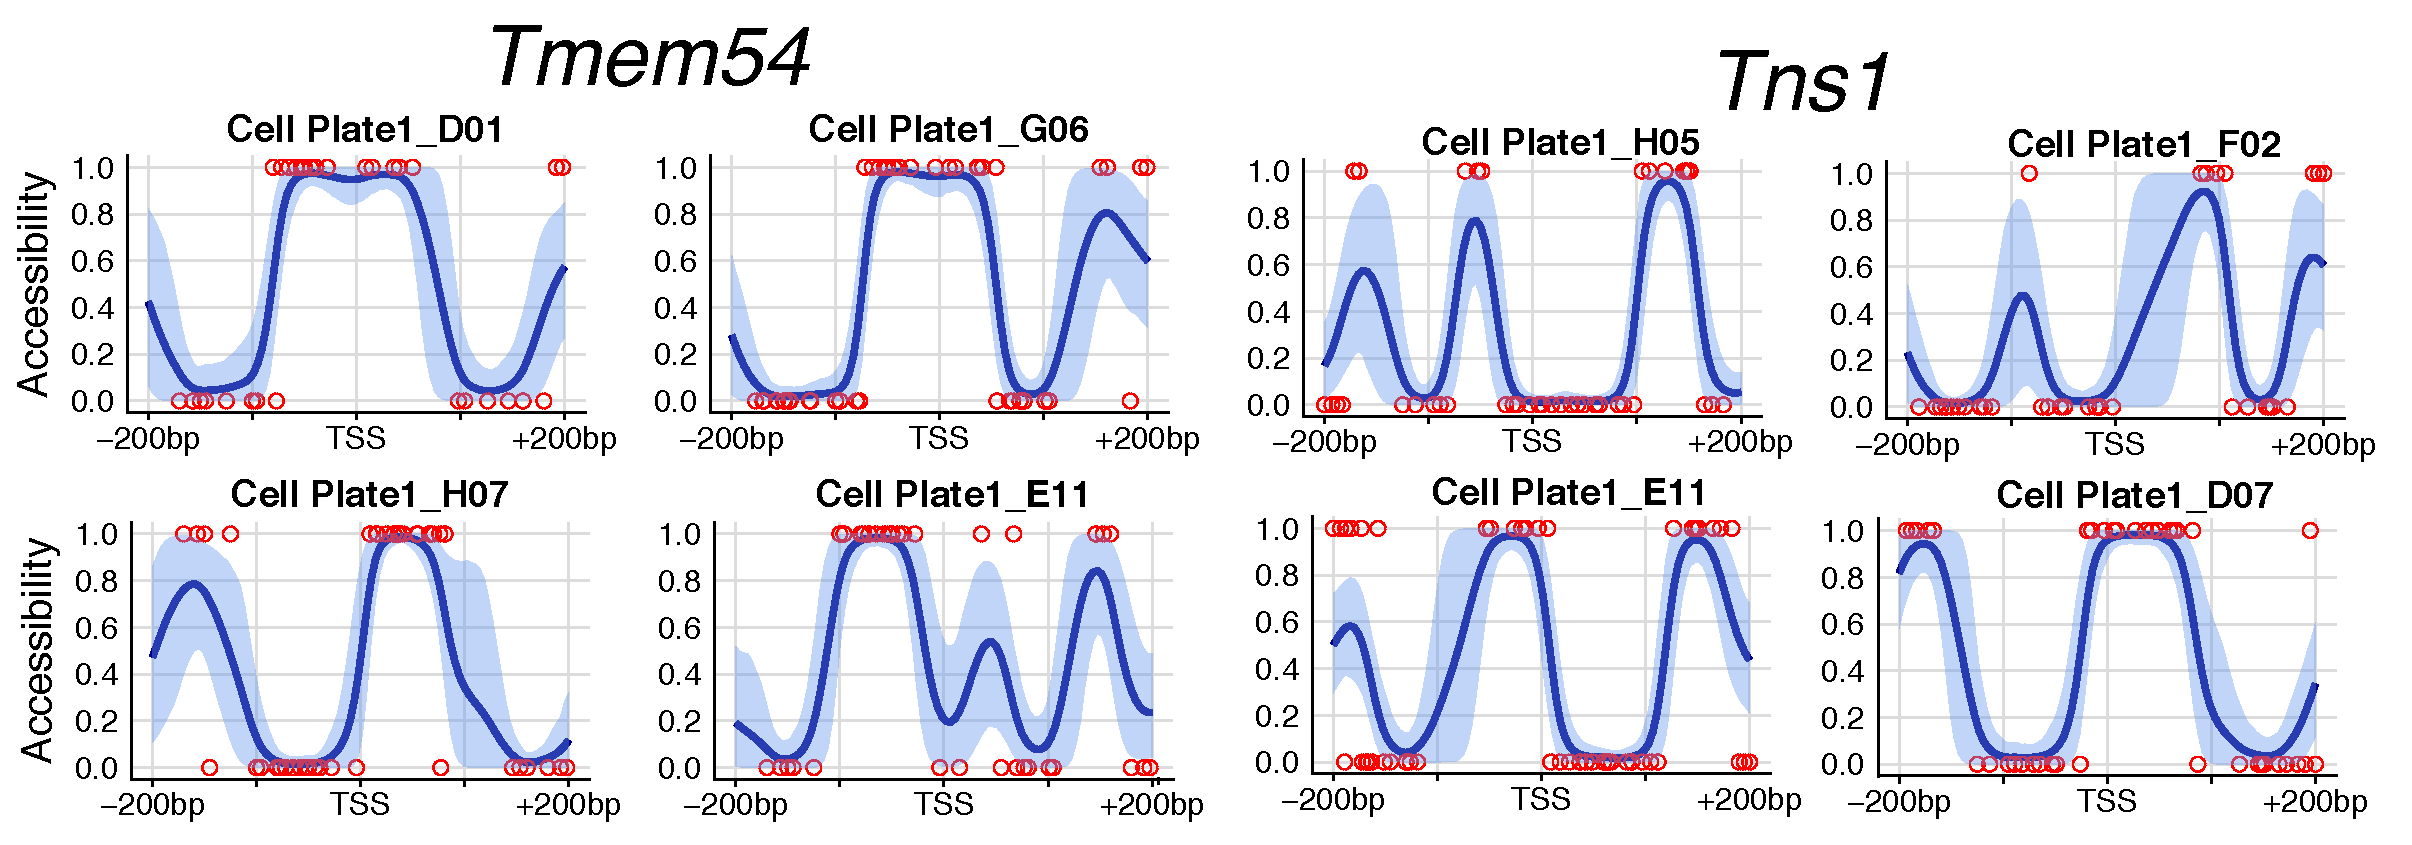
\includegraphics[width=0.9\linewidth]{scNMT_profiles_examples}
	\caption[]{}
	\label{fig:scnmt_profiles_examples}
\end{figure}


As a first validation step, we showed that the accessibility profiles infered around the transcription start site (TSS) lead to a better prediction of RNA expression than using conventional accessibility rates (Figure X).

\begin{figure}[H]
	\centering
	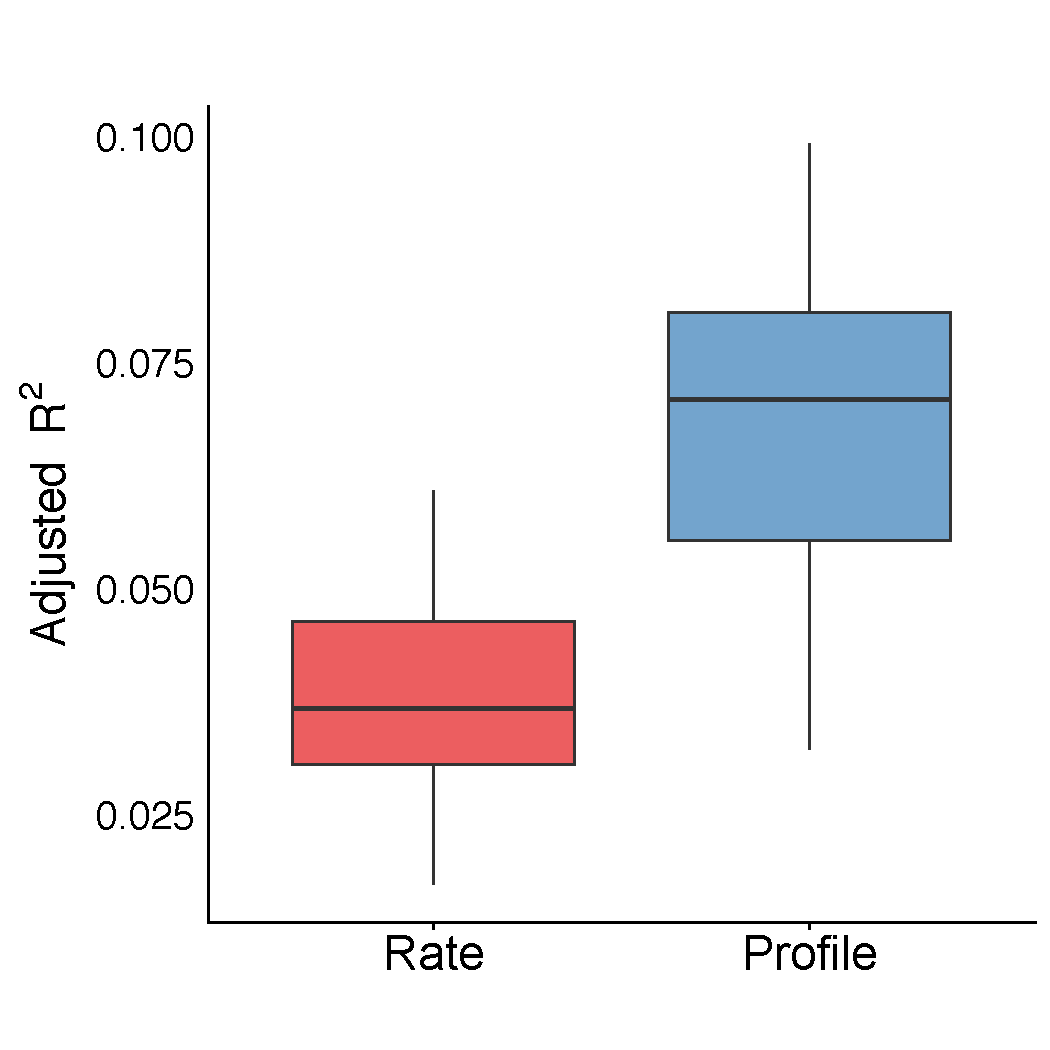
\includegraphics[width=0.65\linewidth]{scNMT_profiles_prediction}
	\caption[]{}
	\label{fig:scnmt_profiles_prediction}
\end{figure}


Consistently, when inspecting individual genes we observe that highly expressed genes show characteristic patterns of nucleosome depleted regions around the TSS, whereas lowly expressed genes show low levels of chromatin accessibility:

\begin{figure}[H]
	\centering
	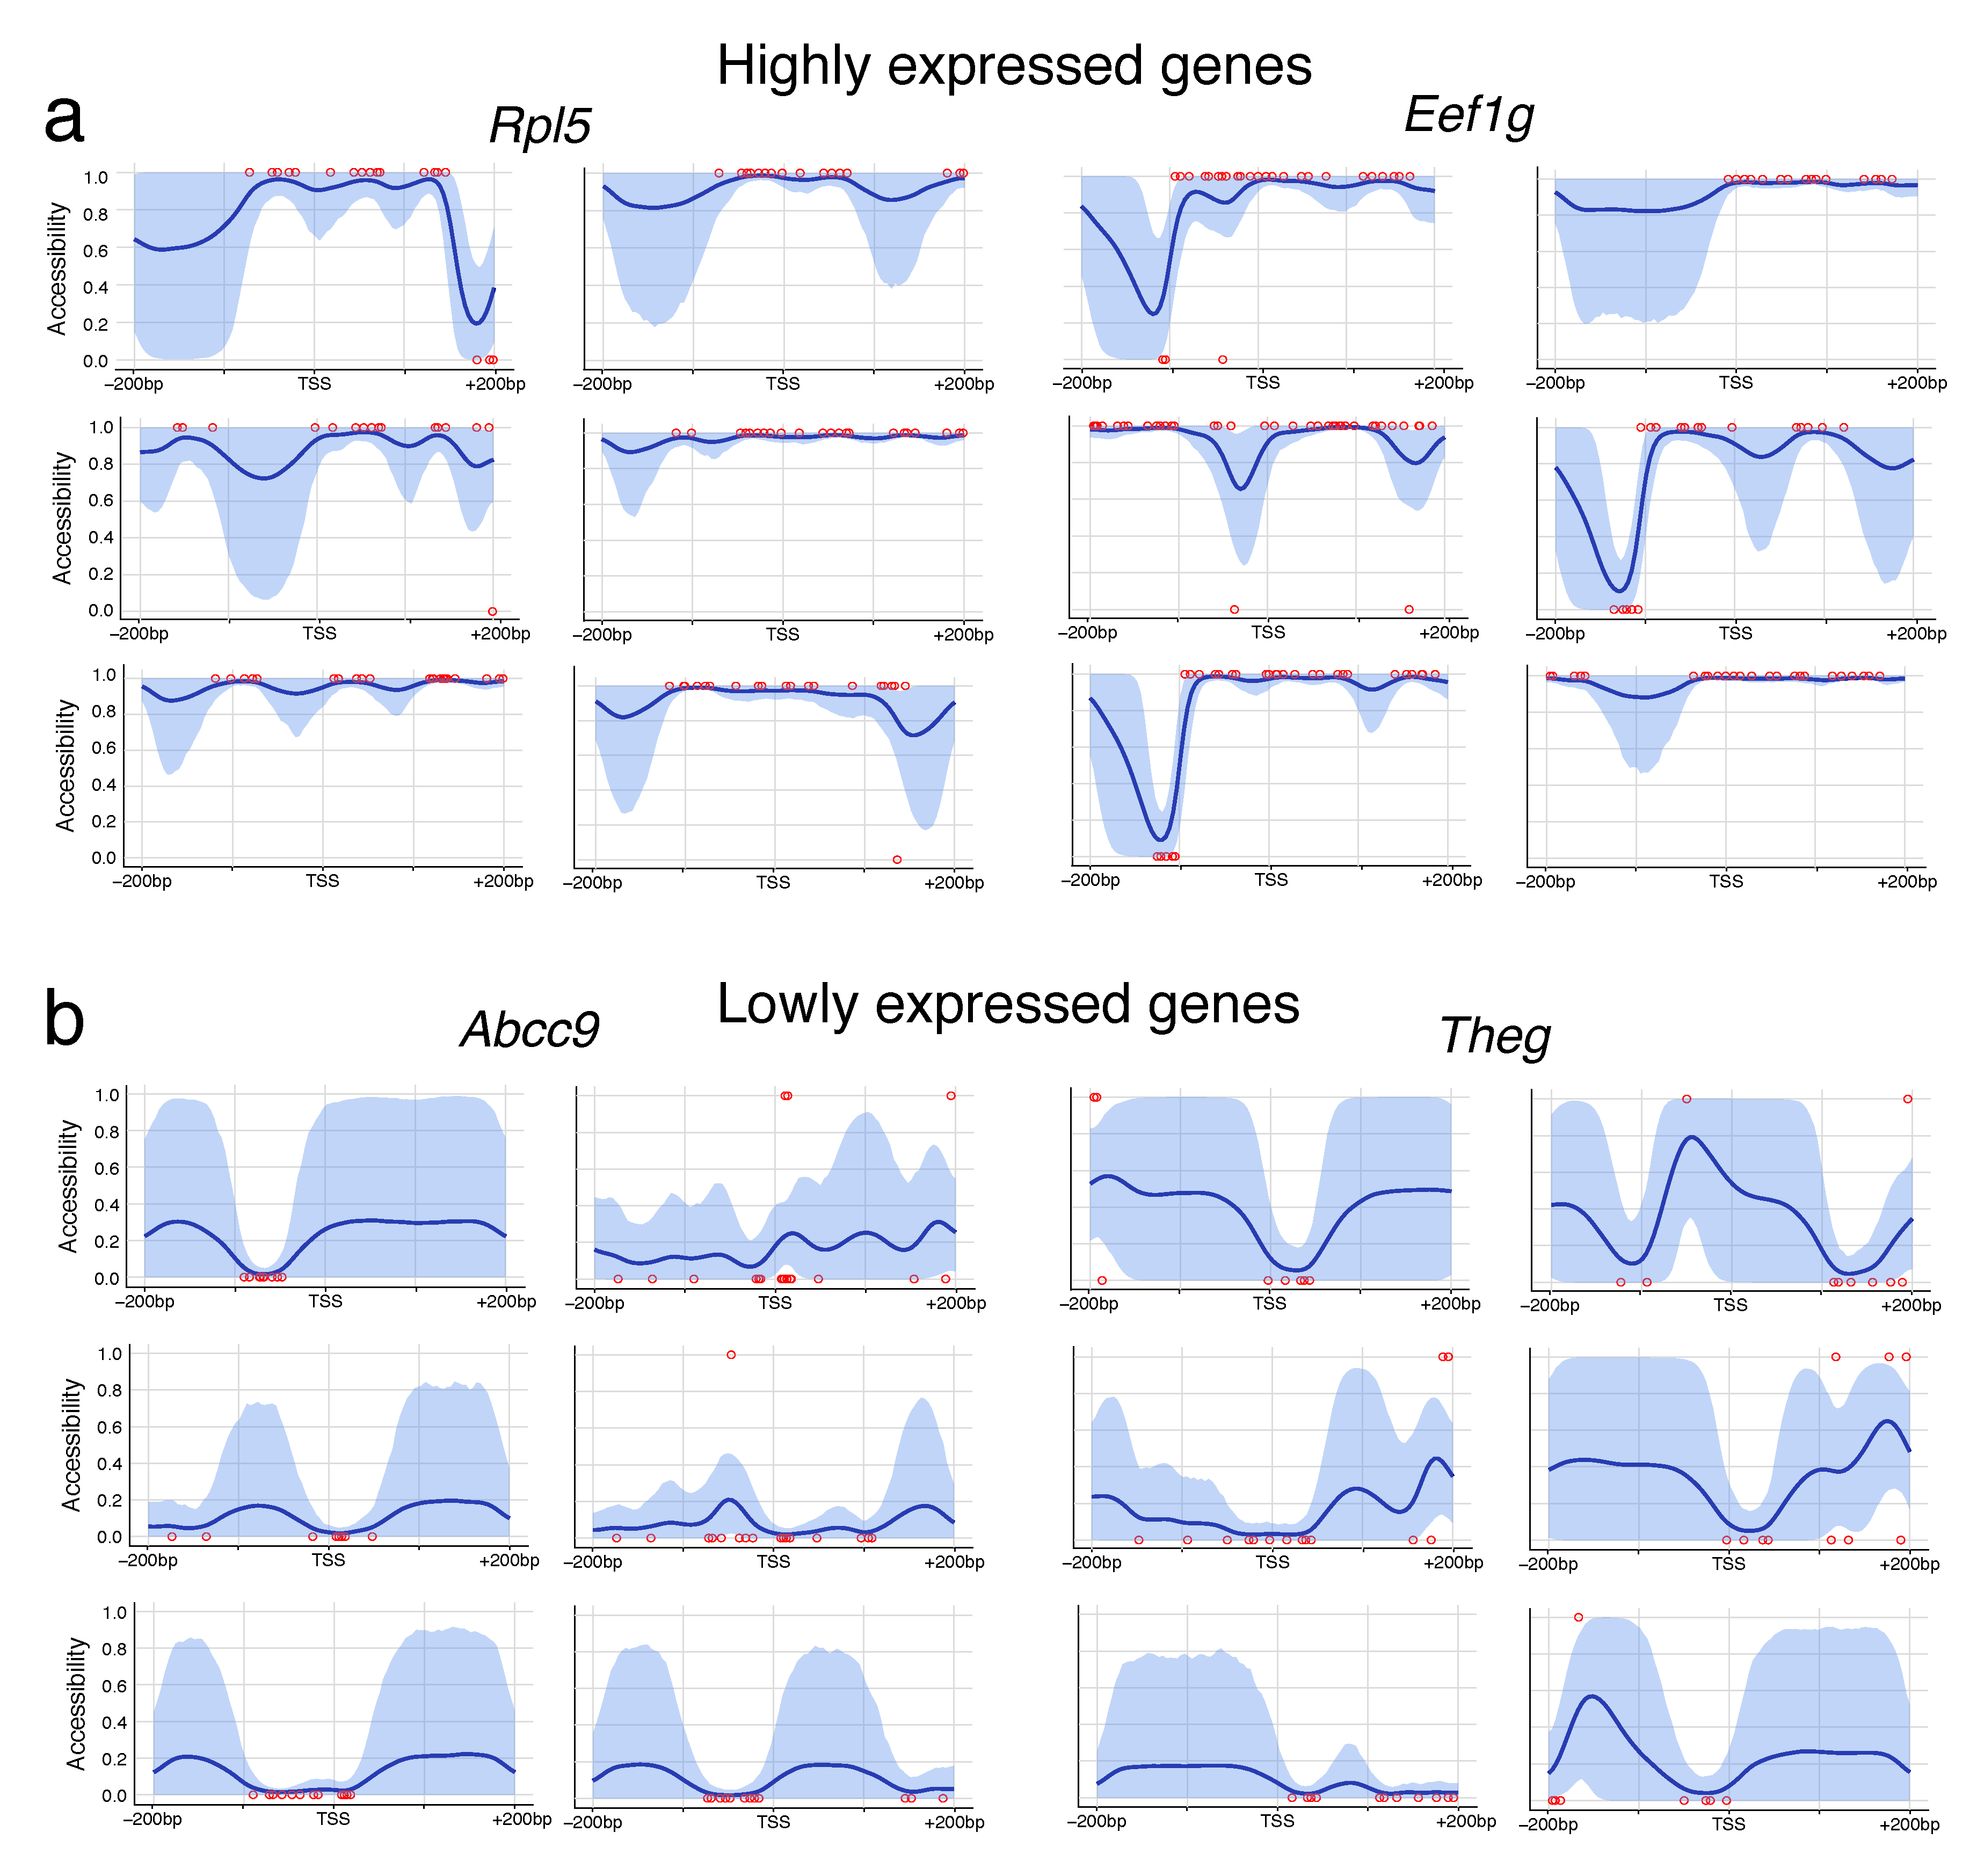
\includegraphics[width=0.9\linewidth]{scNMT_profiles_expr}
	\caption[]{}
	\label{fig:scnmt_profiles_highexpr}
\end{figure}

Next, we attempted at linking the heterogeneity in chromatin accessibility profiles with the variability in RNA expression.\\
A challenge of this augmented representation is how to find a one-dimensional statistic that summarises the heterogeneity across cells (as the variance statistic in conventional rates), which can be in turn correlated with summary statistics from the RNA expression. The approach we followed here is to cluster cells (per gene) based on the similarity of the accessibility profiles, using a finite mixture model with an expectation–maximisation algorithm. The optimal number of clusters was estimated using a Bayesian Information Criterion.\\
After model fitting, we considered the number of clusters as a proxy for accessibility heterogeneity, the rationale being that homogeneous genes will be grouped in a single cluster, while heterogeneous genes will contain a higher number of clusters.\\

\begin{figure}[H]
	\centering
	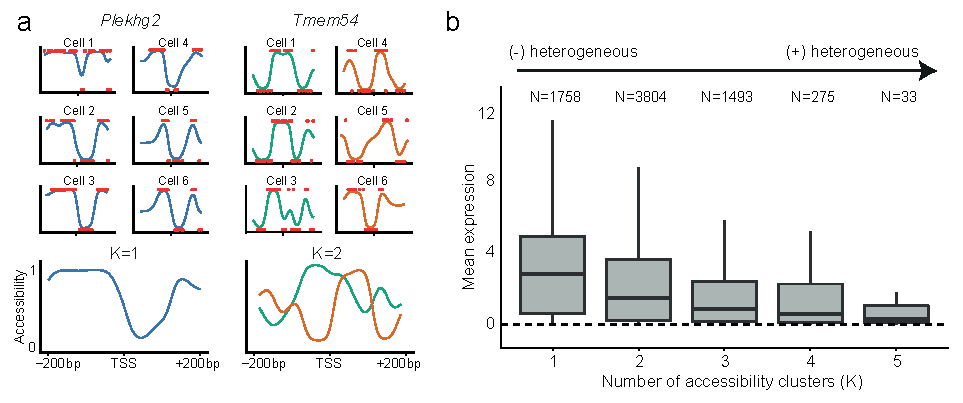
\includegraphics[width=0.9\linewidth]{scNMT_profiles_clusters}
	\caption[]{}
	\label{fig:scnmt_profiles_clusters}
\end{figure}

When relating the number of clusters to the gene expression, we observed that genes with homogeneous accessibility profiles (fewer clusters) were associated with higher average expression levels. Gene Ontology enrichment analysis suggests that this cluster is enriched by genes with houseekeping functions, which are known to display more conserved epigenetic features \cite{She2009}.\\
In contrast, genes with heterogeneous accessibility (multiple clusters) were associated with lower expression levels and were enriched for bivalent domains, containing both active H3K4me3 and repressive H3K27me3 histone marks. As reported in previous studies, bivalent chromatin is normally associated with lowly-expressed genes that are poised for activation upon cell differentiation, thus playing a fundamental role in pluripotency and development \cite{Vastenhouw2012,Bernstein2006}

\begin{figure}[H]
	\centering
	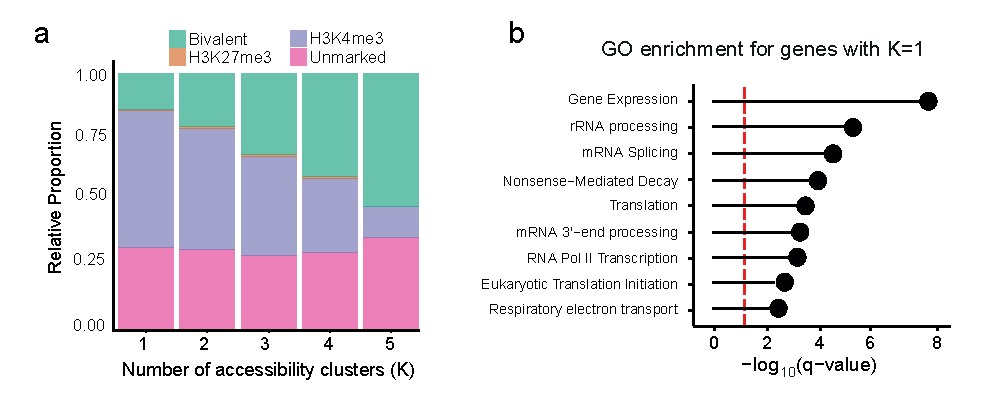
\includegraphics[width=0.9\linewidth]{scNMT_profiles_clusters2}
	\caption[]{}
	\label{fig:scnmt_profiles_clusters2}
\end{figure}




% \begin{figure}[H]
% 	\centering
% 	\includegraphics[width=0.9\linewidth]{scNMT_profiles_clusters_examples}
% 	\caption[]{}
% 	\label{fig:scnmt_profiles_clusters_examples}
% \end{figure}

In conclusion, we have shown that the use of non-linear methods for summarising NOME-seq accessibility data can yield novel insights into the chromatin organisation, nucleosome positioning and the consequent regulation of gene expression. Yet, we acknowledge that this novel methodology needs to be further validated using other data sets, and some improvements need to be implemented in order to ensure that robust biological signal can be extracted from single-cell studies. First, the use of faster inference frameworks, which has been implemented in the new version of the software \cite{Kapourani2018}. Second, the method requires a large number of measurements for an accurate regression. In this study we used relatively lenient thresholds and only \~25\% genes passed coverage filtering. An attempt to improve this could be the use of Bayesian methods that simultaneously cluster and fit the regression model, effectively leveraging information about the similarity between individual cells \cite{Kapourani2018b}. Finally, one could aim at learning a joint model with DNA methylation and chromatin accessiblity to provide an extra layer of multi-modal information.


\section{Characterisation of epigenome dynamics along a developmental trajectory}
The use of single-cell technologies has permitted the unbiased study of continuous trajectories by computationally reconstructing the \textit{pseudotemporal} dynamics from the molecular profiles \cite{Trapnell2014,Haghverdi2016,Saelens2018}. A novel opportunity unveiled by the introduction of single-cell multi-modal technologies is the study of epigenetic dynamics along pseudotime trajectories infered from the transcriptome.\\

To explore this idea, we applied a diffusion pseudotime method from the \textit{destiny} package\cite{Haghverdi2016}, using the RNA expression of the 500 genes with highest biological overdispersion, as estimated by the \textit{scran} package \cite{Lun2016}. The resulting first diffusion component was used to reconstruct a pseudotemporal ordering of cells from pluripotent to differentiated states:

\begin{figure}[H]
	\centering
	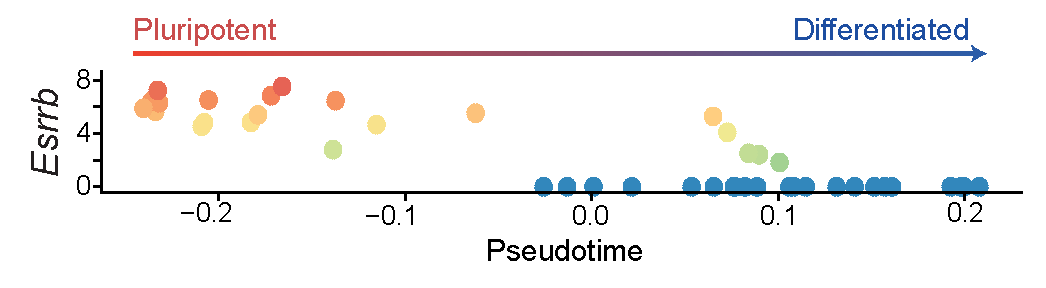
\includegraphics[width=0.9\linewidth]{scNMT_pseudotime}
	\caption[]{}
	\label{fig:scnmt_pseudotime}
\end{figure}


Next, we aimed at identifying genes with coordinated changes in the promoter accessibility and position of the cell in the trajectory using Spearman’s rank coefficient test. This identified 15 significant genes, most of them showing a positive coefficient linked to a decrease in chromatin accessibility along the trajectory.

\begin{figure}[H]
	\centering
	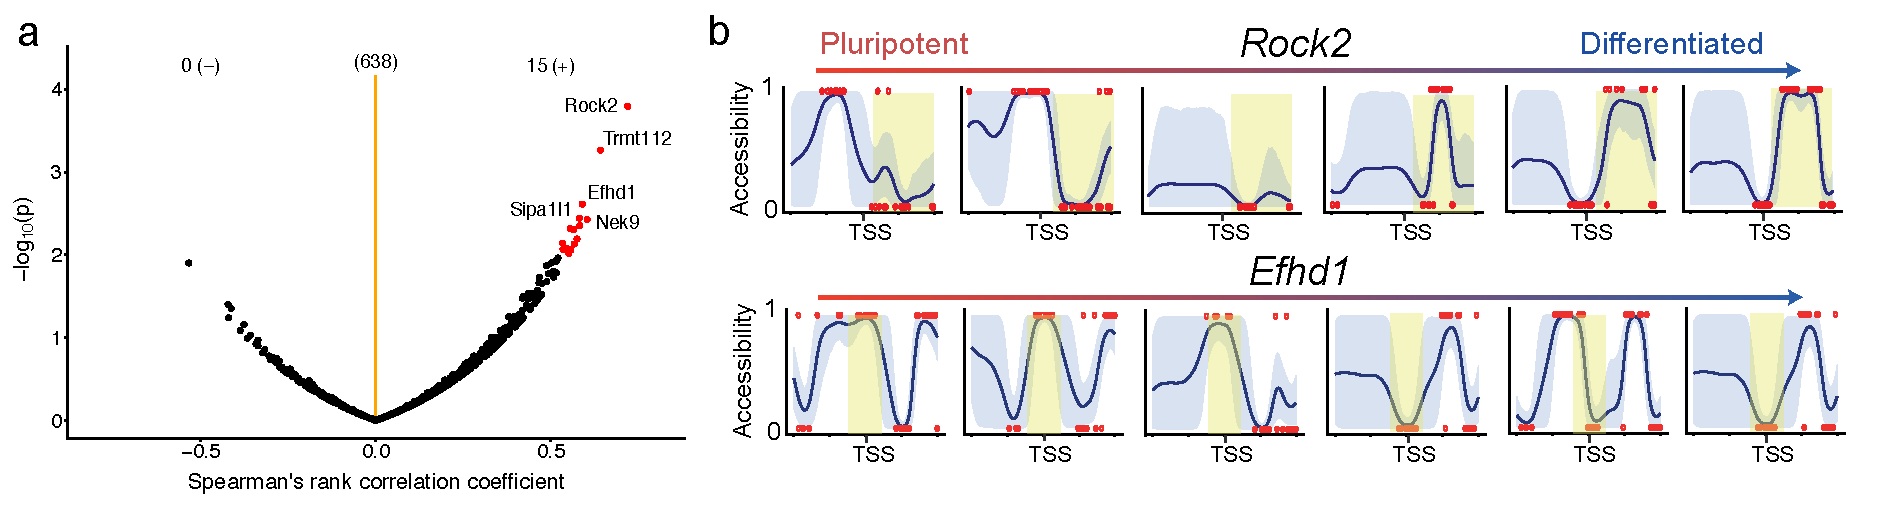
\includegraphics[width=0.9\linewidth]{scNMT_pseudotime_correlation}
	\caption[]{}
	\label{fig:scnmt_pseudotime_correlation}
\end{figure}

%(COPIED) Finally, we investigated whether dynamic changes in the coupling between the epigenetic layers are observed along the differentiation trajectory. To this end, we plotted methylation- accessibility correlation coefficients (as calculated in Fig. 2a) against pseudotime, which revealed an increasing negative correlation coefficient between DNA methylation and accessi- bility in practically all genomic contexts (Fig. 5c). Notably, this suggests that the coupling between the epigenetic layers increases as cells commit to downstream lineages, which could be an important step in lineage priming. Importantly, this analysis was made possible by the continuous nature of the single-cell pseudotime ordering and the ability to profile the three molecular layers and highlights the utility of such parallel single-cell techniques.


\begin{figure}[H]
	\centering
	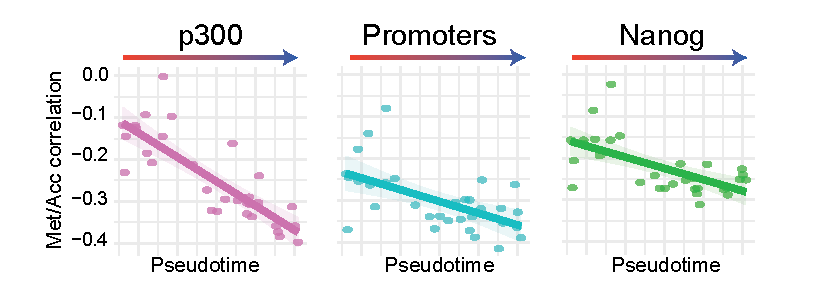
\includegraphics[width=0.9\linewidth]{scNMT_pseudotime_coupling}
	\caption[]{}
	\label{fig:scnmt_pseudotime_coupling}
\end{figure}

\section{Open perspectives}
Scalability
Intron counts and RNA velocity
Infering genomic information
Imputation 
Exploration of non-linear profiles
Further validartion and application to new data sets

